\section{Chapter 6 Proposed Framework and System Architecture}

\subsection{6.1 Introduction}

Based on the limitations identified in the previous chapters, this research proposes CloudSentinel AI, a context-aware cloud security framework designed to enhance traditional Cloud Security Posture Management (CSPM). Unlike existing solutions that primarily evaluate cloud resources independently, the proposed framework correlates cloud assets, security configurations, identities, and network relationships to provide a comprehensive assessment of the cloud security posture. The proposed framework combines automated cloud asset discovery, rule-based security validation, graph-based resource modeling, attack path generation, contextual risk assessment, and Explainable Artificial Intelligence (XAI) into a unified architecture. This integration enables security analysts to understand not only which cloud resources are misconfigured but also how multiple weaknesses can interact to create exploitable attack paths. The overall architecture of the proposed CloudSentinel AI framework is illustrated in Figure 6.1. The architecture is organized into modular components, each responsible for a specific stage of the cloud security assessment process. This modular design improves scalability, maintainability, and extensibility while allowing future integration with additional cloud providers and security technologies.

\begin{figure}
\hypertarget{fig:6_1}{%
\centering
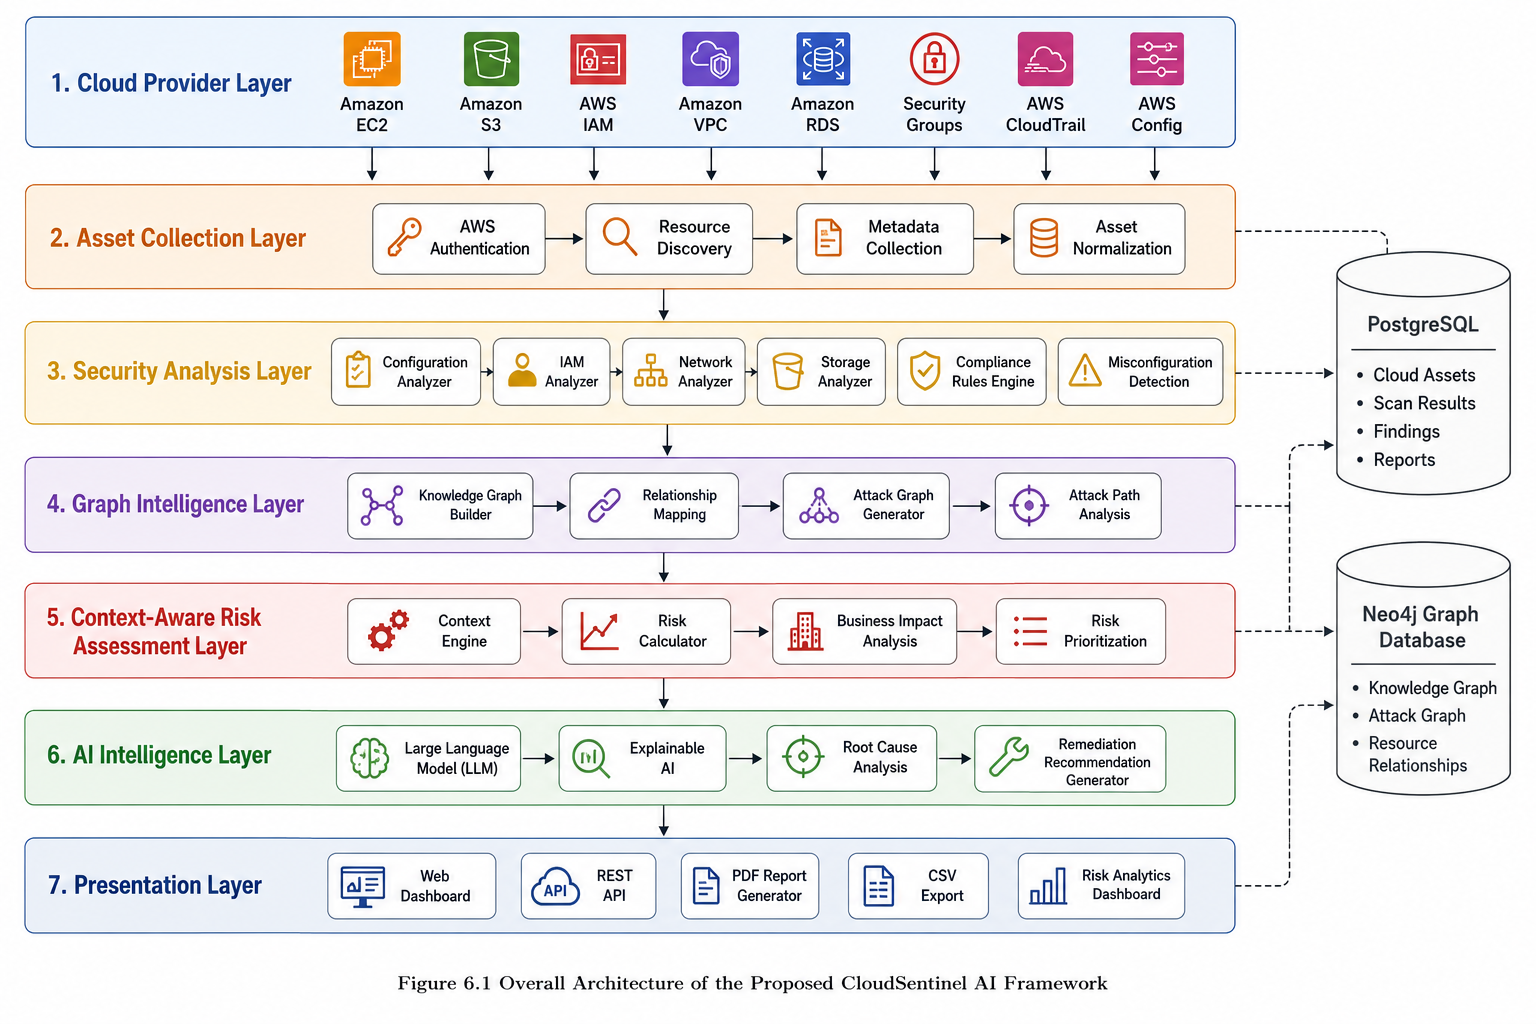
\includegraphics[width=0.9\textwidth,height=\textheight]{figures/image-6.1.png}
\caption{CloudSentinel AI System Architecture.}\label{fig:6_1}
}
\end{figure}

\subsection{6.2 Design Objectives}

The proposed framework has been designed with the following objectives:\\
\#\#\# 6.2.1 Automated Cloud Asset Discovery: The framework should automatically discover cloud resources by interacting with cloud provider APIs without requiring manual inventory creation. \#\#\# 6.2.2 Context-Aware Security Analysis: The framework should analyze relationships among identities, storage services, virtual machines, databases, networking components, and security policies to determine the overall security posture. \#\#\# 6.2.3 Attack Path Identification: The framework should identify possible attack paths by correlating multiple cloud misconfigurations. \#\#\# 6.2.4 Dynamic Risk Prioritization: Risk assessment should consider contextual information such as asset criticality, identity permissions, network exposure, and business impact instead of relying solely on predefined severity levels. \#\#\# 6.2.5 Explainable Security Recommendations: The framework should provide human-readable explanations describing detected security risks, possible attack scenarios, and recommended mitigation strategies. \#\#\# 6.2.6 Extensible System Design: The architecture should support future enhancements such as multi-cloud environments, Kubernetes security, Infrastructure-as-Code validation, and real-time security monitoring.

\subsection{6.3 Overall System Architecture}

CloudSentinel AI follows a modular architecture where each component performs a dedicated function while contributing to the overall security assessment process. The architecture consists of eight major modules that work together to transform raw cloud configuration data into actionable security intelligence. The overall workflow begins with cloud asset discovery, followed by configuration analysis, knowledge graph construction, attack path generation, context-aware risk engine processing, and explainable AI generation.

\subsection{6.4 Functional Modules of CloudSentinel AI}

\subsubsection{6.4.1 Cloud Asset Collector: Retrieves metadata regarding cloud resources directly from cloud provider APIs (e.g., AWS EC2, S3, IAM, VPC).}

\subsubsection{6.4.2 Configuration Analyzer: Evaluates resources against predefined security rules (e.g., public S3 buckets, overly permissive IAM, open security groups).}

\subsubsection{6.4.3 Knowledge Graph Builder: Transforms the cloud environment into an interconnected network, representing resources as nodes and relationships as edges.}

\subsubsection{6.4.4 Rule Engine: Evaluates cloud configurations using rules derived from CIS AWS Benchmarks, AWS Well-Architected Framework, and NIST guidelines.}

\subsubsection{6.4.5 Attack Graph Generator: Analyzes the knowledge graph to identify potential attack paths by correlating multiple cloud resources and security weaknesses.}

\subsubsection{6.4.6 Context-Aware Risk Engine: Calculates dynamic risk scores using factors like asset criticality, network exposure, and identity privileges.}

\subsubsection{6.4.7 Explainable AI Module: Generates human-readable explanations describing identified security issues, attack progression, and recommended remediation.}

\subsubsection{6.4.8 Dashboard and Reporting Module: Provides an interactive interface for visualizing security findings, attack paths, and risk scores.}

\subsection{6.5 Workflow of the Proposed Framework}

The operational workflow begins with cloud resource collection. Metadata is processed by the Configuration Analyzer and Rule Engine. The Knowledge Graph Builder then maps the environment, and the Attack Graph Generator identifies exploitation paths. These paths are evaluated by the Context-Aware Risk Engine, and the Explainable AI module provides remediation guidance through the Dashboard.

\subsection{6.6 Design Advantages of the Proposed Framework}

\begin{itemize}
\tightlist
\item
  Correlates cloud resources instead of analyzing them independently.\\
\item
  Generates attack paths representing realistic exploitation scenarios.\\
\item
  Utilizes graph-based reasoning for security assessment.\\
\item
  Performs contextual risk evaluation instead of static severity classification.\\
\item
  Provides Explainable AI-generated security recommendations.\\
\item
  Reduces alert fatigue by prioritizing exploitable attack chains.\\
\item
  Supports future extension to multi-cloud and cloud-native environments.
\end{itemize}

\subsection{6.7 Chapter Summary}

This chapter presented the CloudSentinel AI framework, detailing its modular architecture, design objectives, and operational workflow. By integrating graph-based modeling with AI-assisted security analysis, the proposed framework addresses the limitations identified in existing CSPM and CNAPP solutions. The next chapter details the research methodology, implementation strategy, and evaluation approach.

\subsection{Additional Figures}

\begin{figure}
\hypertarget{fig:6_2}{%
\centering
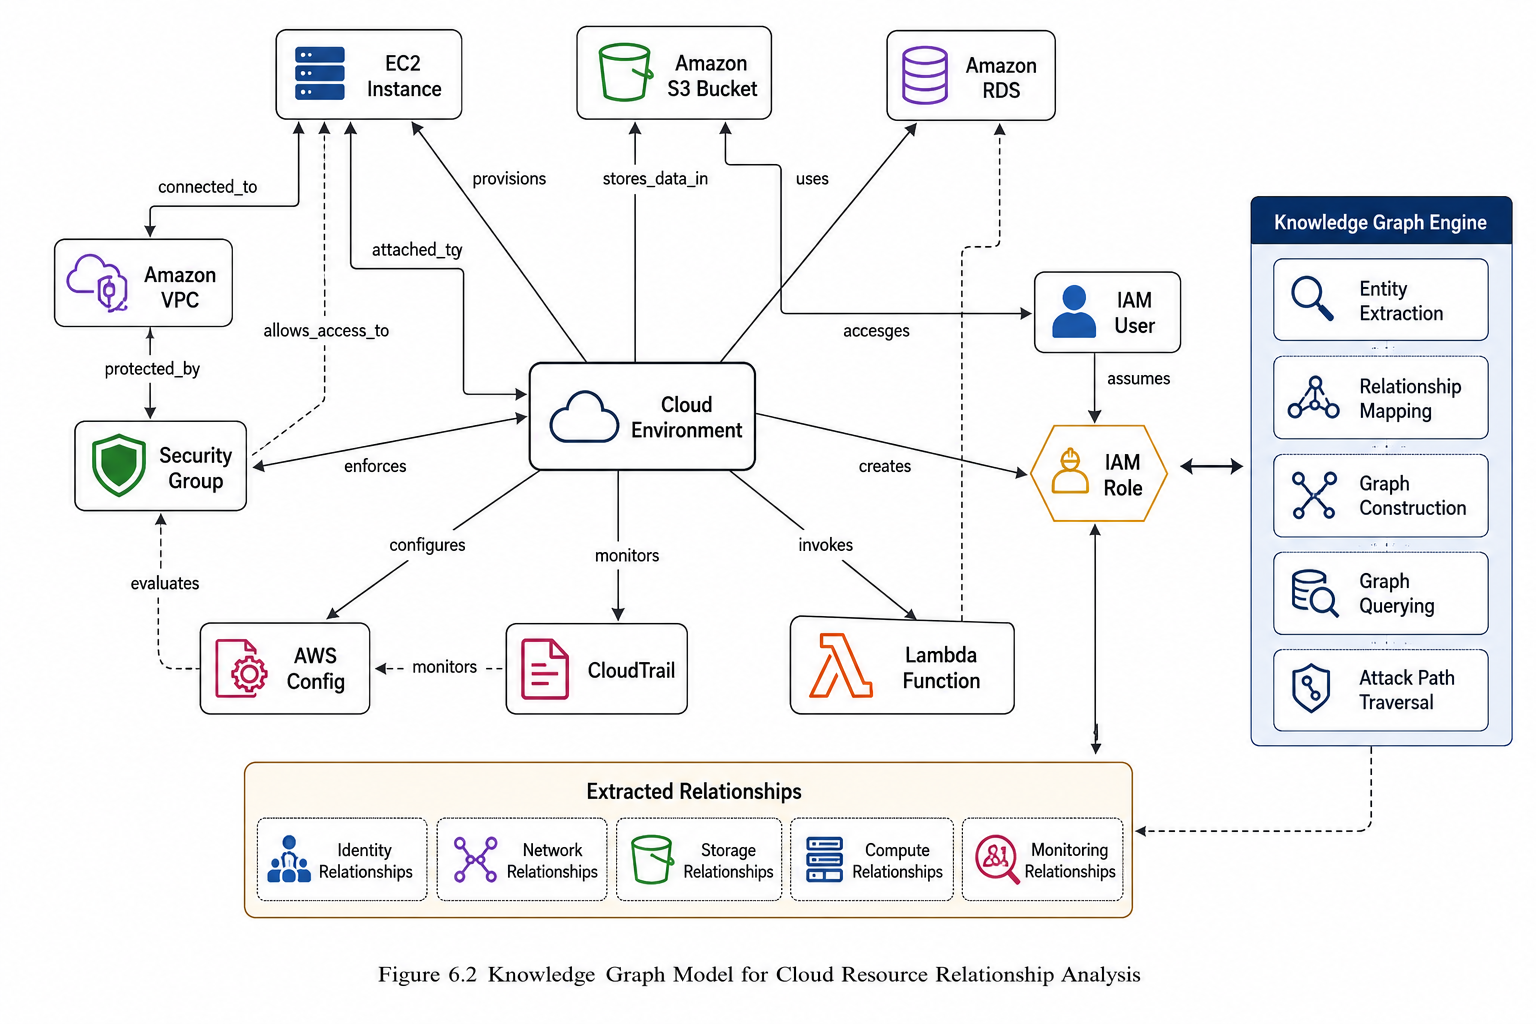
\includegraphics[width=0.9\textwidth,height=\textheight]{figures/image-6.2.png}
\caption{Cloud Asset and Security Analysis Workflow.}\label{fig:6_2}
}
\end{figure}

\begin{figure}
\hypertarget{fig:6_3}{%
\centering
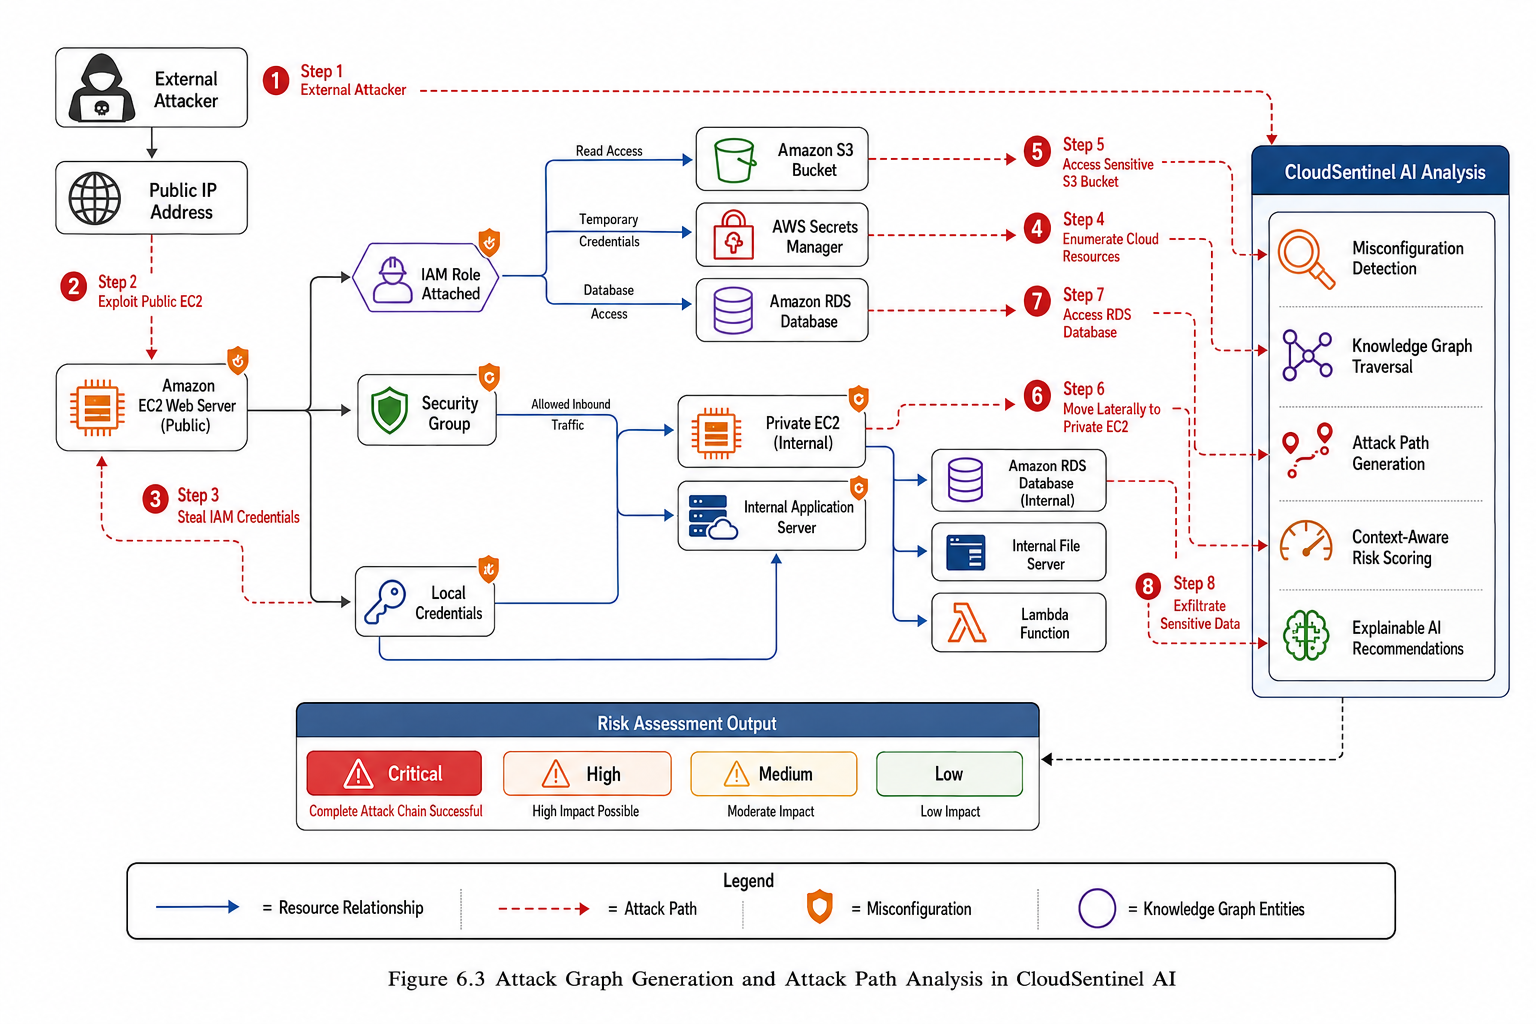
\includegraphics[width=0.9\textwidth,height=\textheight]{figures/image-6.3.png}
\caption{Knowledge Graph Construction Pipeline.}\label{fig:6_3}
}
\end{figure}

\begin{figure}
\hypertarget{fig:6_4}{%
\centering
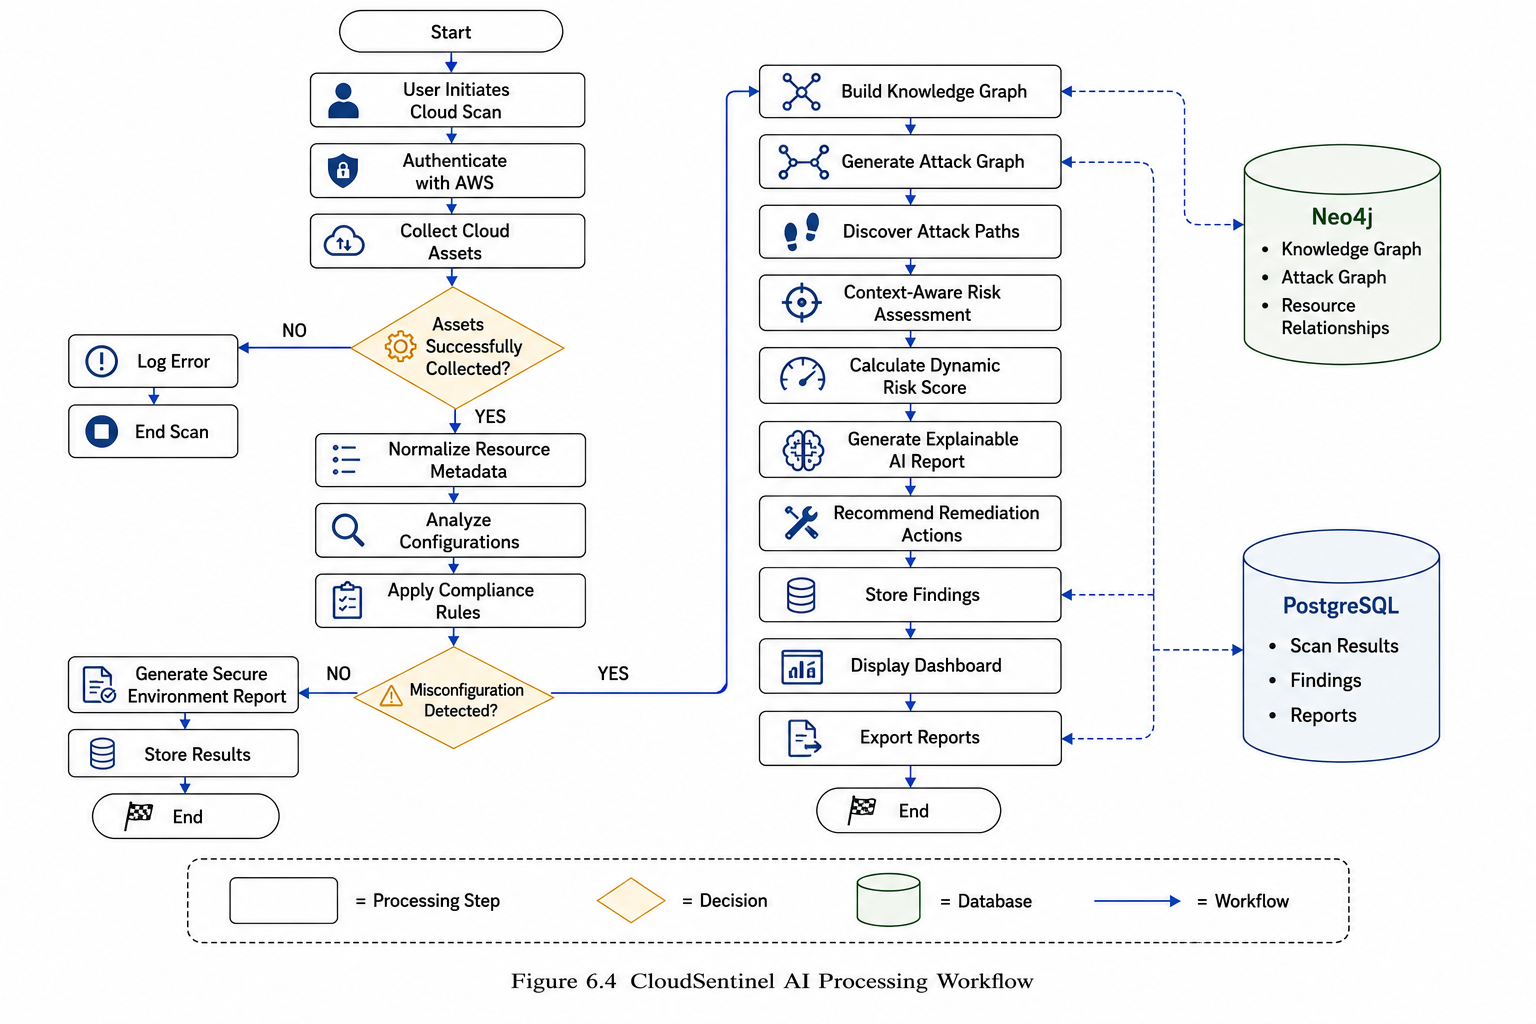
\includegraphics[width=0.9\textwidth,height=\textheight]{figures/image-6.4.png}
\caption{Context-Aware Risk Assessment Flow.}\label{fig:6_4}
}
\end{figure}
